%!TEX TS-program = xelatex
%Time-stamp: 10/25/2012 3:51:45 PM
\documentclass[openany,reqno]{amsbook}
\input ../preamble
\newcommand\version{1.0}
\newcommand\semester{Fall 2012}
%%%%%%%%%%%%%%%%%%%%%%%%%%%%%%%%%%%%%
%\includeonly{09intapps}
%%%%%%%%%%%%%%%%%%%%%%%%%%%%%%%%%%%%%
\begin{document}
\graphicspath{{figures/}}
\section*{Answers and Hints}
\begin{trivlist}\problemfont
  %\footnotesize
  \setlength{\parindent}{0pt}
  \setlength{\parskip}{0.5ex plus0.5ex}
  \raggedright
  \relax
  \tolerance10000



\item[{\bf(I2.1)}]

  The decimal expansion of
  \[
    1/7 = 0.\overline{142857}\,142857\,142857\,\cdots
  \]
  repeats after 6 digits.  Since $2007 =
  334\times6+3$ the $2007^{\textrm{th}}$ digit is the same as the
  $3^{\textrm{rd}}$, which happens to be a $2$.
  \bigskip

\item[{\bf(I2.5)}]

  Yes these are the same sets.  Both sets consist of all positive real
  numbers: since they contain exactly the same numbers, they are the
  same sets.
  \bigskip

\item[{\bf(I2.6)}]

  $100x = 31.313131\cdots = 31+x \implies 99x = 31 \implies x =
  \frac{31}{99}$.

  Similarly, $1000y = 273 + y$ so $y= \frac{273}{999}$.

  In $z$ the initial ``$2$'' is not part of the repeating pattern, so
  subtract it:  $z = 0.2 + 0.0154154154\cdots$.  Now let
  $w=0.0154154154\cdots$.  You get $1000w = 15.4+w = 15\frac25 + w =
  \frac{77}{5}+w$. Therefore $w= \frac{77}{5\times 999}$.
  From this you get
  \[
    z = \tfrac15+w = \tfrac15 +  \frac{77}{5\times999} = \frac{1076}{4995}.
  \]
  \bigskip

\item[{\bf(I7.1)}]

  They are the same function.  Both are defined for all real numbers,
  and both will square whatever number you give them, so they are the
  same function.
  \bigskip

\item[{\bf(I7.4)}]

  Let $x$ be any number.  Then, $f(x)$, if it is defined, is the largest

  \bigskip

\item[{\bf(I7.6)}]

  The domain of $k^{-1} $ is $(0, \infty)$, and $k^{-1}(x) = -\sqrt{x}$.
  \bigskip

\item[{\bf(I7.8a)}]

  False: Since $\arcsin x$ is only defined if $-1\leq x\leq 1$ and hence
  not for \emph{all} $x$, it is not true that $\sin\bigl(\arcsin
  x\bigr) = x$ for \emph{all} real numbers $x$.
  However, it is true that $\sin(\arcsin x) = x$ for all $x$ in
  the interval $[-1,1]$.
  \bigskip

\item[{\bf(I7.8b)}]

  $\arcsin(\sin x)$ is defined for all $x$ since $\sin x$ is
  defined for all $x$, and $\sin x$ is always between $-1$ and $1$.
  However the arcsine function always returns a number (angle) between
  $-\pi/2$ and $\pi/2$, so $\arcsin( \sin x) = x$ can't be true when
  $x>\pi/2$ or $x<-\pi/2$.  For $|x|\leq \pi/2$ it is true that $\arcsin
  \sin x = x$.
  \bigskip

\item[{\bf(I7.8c)}]

  Again, not true: if $x=\pi/2$ then $\tan x$ is not defined and therefore
  $\arctan(\tan x)$ is not defined either.

  Apart from that, $\arctan (\text{anything})$ always lies
  between $-\pi/2 $ and $+\pi/2$, so $\arctan(\tan x)$ cannot
  be the same as $x$ if either $x>\pi/2$ or $x<-\pi/2$.
  \bigskip

\item[{\bf(I7.8d)}]

  True.
  \bigskip

\item[{\bf(I7.14a)}]

  Set $x=-3/2$ in $f(2x+3) = x^2$ and you find $f(0) = (-3/2)^2 =
  \frac{9}{4}$.
  \bigskip

\item[{\bf(I7.14b)}]

  Set $x=0$ in $f(2x+3) = x^2$ and you find $f(3) = 0^2 = 0$.
  \bigskip

\item[{\bf(I7.14c)}]

  Solve $2x+3 = t$ for $x$:  $x=\frac{t-3}{2}$.  Substitute this in $f(2x+3) =
  x^2$ and you find $f(t) = \bigl(\frac{t-3}{2}\bigr)^2$.
  \bigskip

\item[{\bf(I7.14d)}]

  From the previous problem we know what $f(t)$ is for any $t$ so just substitute $t=x$:
  $f(x)= b\bigl(\frac{x-3}{2}\bigr)^2$.

  \bigskip

\item[{\bf(I7.14e)}]

  $f(2) = \bigl((2-3)/2\bigr)^2 = \frac{1}{4}$.
  \bigskip

\item[{\bf(I7.14f)}]

  $f(2f(x)) = \bigl(\frac{2f(x)-3}{2}\bigr)^2 =
  \Bigl\{\frac{2\bigl(\frac{x-3}{2}\bigr)^2 - 3}{2}\Bigr\}^2$.

  \bigskip

\item[{\bf(I7.15a)}]

  We know $f\bigl(\frac1{x+1}\bigr) = 2x-12$ for all $x$, so if we want to know
  $f(1)$ then we have to find an $x$ with $\frac{1}{x+1} = 1$.  Solving $\frac{1}{x+1} = 1$
  for $x$ you find $x=0$. Substitute $x=0$ in $f\bigl(\frac1{x+1}\bigr) = 2x-12$
  and you get $f(1) = 2\times0-12 = -12$.
  \bigskip

\item[{\bf(I7.15b)}]

  To find $f(0)$ you proceed as above, this time solving $\frac{1}{x+1} = 0$ for
  $x$.  In this case there is no solution $x$, and therefore the equation
  $f\bigl(\frac1{x+1}\bigr) = 2x-12$ does not tell us what $f(0)$ is.  Conclusion:
  either 0 is not in the domain of $f$, or we cannot tell what $f(0)$ is from
  the  information provided in the problem.
  \bigskip

\item[{\bf(I7.15c)}]

  To find $f(t)$ you do the same as when you want to find $f(1)$.
  We know $f\bigl(\frac1{x+1}\bigr) = 2x-12$ for all $x$, so if we want to know
  $f(t)$ then we have to find an $x$ with $\frac{1}{x+1} = t$.  Solving $\frac{1}{x+1} = t$
  for $x$ you find $x=\frac 1t -1$. Substitute $x=\frac 1t -1$ in $f\bigl(\frac1{x+1}\bigr) = 2x-12$
  and you get $f(t) = 2\times\bigl(\frac{1}{t}-1\bigr)-12 = \frac{2}{t} -14 $.
  \bigskip

\item[{\bf(I7.15d)}]

  $f(2f(x)) = \frac{2}{2f(x)} - 14 = \frac{1}{f(x)} - 14 =
  \frac{1}{\frac{2}{x}-14} - 14$.  You could simplify this if you wanted to, but
  that was not part of the question.
  \bigskip

\item[{\bf(I7.15e)}]

  After finding $f(t) = \frac{2}{t} -14 $ you can substitute $t=x$ and you find
  $f(x) = \frac{2}{x} -14 $.
  \bigskip

\item[{\bf(I7.15f)}]

  $f(2) = \frac{2}{2}-14 = -13 $ and therefore $f(f(2)) = f(-13) = \frac{2}{-13}-14 = -14\frac2{13} $.
  \bigskip

\item[{\bf(I7.16)}]

  No.  For instance if you set $x=1$ you get $f(1) = 1+1=2$, and if you set
  $x=-1$ then you get $f((-1)^2) = (-1)+1$, i.e.\ $f(1) = 0$.  But $f(1)$
  can't be equal to both $2$ and $0$, the formula $f(x^2) = x+1$ cannot be
  true for all real numbers $x$.
  \bigskip

\item[{\bf(I7.18)}]

  $g(x) = -2\bigl(x^2-2x\bigr)
  = -2\bigl(x^2-2x+1 -1\bigr)
  = -2\bigl[(x-1)^2 -1\bigr]
  =-2(x-1)^2 + 2$, so the range of $g$ is $(-\infty, 2]$.

  Alternatively:

  $y = g(x) \iff y = -2x^2+4x \iff 2x^2-4x+y = 0$.
  The quadratic formula says that the solutions are
  \[
    x= \frac{4\pm\sqrt{16-8y}} {4}.
  \]
  If $16-8y<0$ then there are no solutions and $y$ does
  not belong to the range of $g$.

  If $16-8y\geq0$ then there is at least one solution
  and  $y$ does belong to the range of $g$.

  Conclusion, the range of $g$ consists of all $y$ with
  $16-8y\geq 0$, i.e.~ all $y\leq2$.
  \bigskip

\item[{\bf(II6.3)}]

  \textbf{(a)}
  \begin{align*}
    \Delta y &= (x+\Delta x)^2  -2 (x+\Delta x)+1 - [x^2-2x+1]\\
    &=(2x-2)\Delta x +(\Delta x)^2 \text{ so that}\\
    \frac{\Delta y}{\Delta x}&= 2x-2 + \Delta x
  \end{align*}
  \bigskip

\item[{\bf(II6.4a)}]

  In this picture $s(t)$ is on the horizontal axis and $t$ is on the vertical axis, so
  horizontal and vertical have been swapped. This curve should pass the \emph{horizontal
  line test}, which it does.
  \bigskip

\item[{\bf(II6.4b)}]

  With a ruler I tried to draw the closest tangent lines at
  the four different times.  Then I measured the slope of those
  four lines using the grid.
  \bigskip

\item[{\bf(II6.5)}]

  At $A$ and $B$ the graph of $f$ is tangent to the drawn lines, so
  the derivative at $A$ is $-1$ and ther derivative at $B$ is $+1$.
  \bigskip

\item[{\bf(II6.6)}]

  $\Delta x$ : feet.  $\Delta y$ pounds. $\frac{\Delta y}{\Delta x}$
  and $\frac{dy}{dx}$ are measured in pounds per feet.
  \bigskip

\item[{\bf(II6.7)}]

  Gallons per second.
  \bigskip

\item[{\bf(II6.8b)}]

  (a) $A(x)$ is an area so it has units square inch and $x$ is
  measured in inches, so $\dfrac{dA}{dx}$ is measured in
  $\displaystyle\frac{\text{inch}^2}{\text{inch}} = \text{inch}$.

  \input figures/02triangleareagrowth.tex


  (b) Hint: The extra area $\Delta A$ that you get when the side of
  an equilateral triangle grows from $x$ to $x+\Delta x$ can be
  split into a thin parallelogram and a very tiny triangle.  Ignore
  the area of the tiny triangle since the area of the parallelogram
  will be much larger.  What is the area of this parallelogram?

  The area of a parallelogram is ``base time height'' so here it is
  $h\times\Delta x$, where $h$ is the height of the triangle.

  Conclusion: $\displaystyle \frac{\Delta A}{\Delta x}
  \approx\frac{h\Delta x}{\Delta x} = h$.

  The derivative is therefore the height of the triangle.

  \bigskip

\item[{\bf(III4.3)}]

  The equation \eqref{eq:derivative-defined-first-time} already
  contains a function $f$, but that is not the right function.  In
  \eqref{eq:derivative-defined-first-time} $\Delta x$ is the variable,
  and $g(\Delta x) = (f(x+\Delta x)-f(x))/\Delta x$ is the function; we
  want $\lim_{\Delta x\to 0}g(\Delta x)$.
  \bigskip

\item[{\bf(III4.4)}]

  $\delta = \varepsilon/2$.
  \bigskip

\item[{\bf(III4.5)}]

  $\delta = \min \bigl\{1, \frac16\varepsilon\bigr\}$
  \bigskip

\item[{\bf(III4.6)}]

  $|f(x) - (-7) |=|x^2-7x+10| = |x-2|\cdot|x-5| $.  If you choose
  $\delta\leq 1$ then $|x-2|<\delta$ implies $1<x<3$, so that $|x-5|$
  is at most $|1-5| = 4$.

  So, choosing $\delta\leq 1$ we always have $|f(x) - L|<4|x-2|$ and
  $|f(x) - L|<\varepsilon$ will follow from $|x-2|<\frac14\varepsilon$.

  Our choice is then: $\delta = \min \bigl\{1, \frac14\varepsilon
  \bigr\}$.
  \bigskip

\item[{\bf(III4.7)}]
  $f(x) = x^3$, $a=3$, $L=27$.

  When $x=3$ one has $x^3=27$, so $x^3-27=0$ for $x=3$.  Therefore you
  can factor out $x-3$ from $x^3-27$ by doing a long division.  You get
  $x^3-27 = (x-3)(x^2+3x+9)$, and thus
  \[
    |f(x) - L| = |x^3-27| =|x^2+3x+9|\cdot|x-3|.
  \]
  Never choose $\delta>1$.  Then $|x-3|<\delta$ will imply $2<x<4$ and
  therefore
  \[
    |x^2+3x+9| \leq 4^2+3\cdot4+9 = 37.
  \]
  So if we always choose $\delta\leq 1$, then we will always have
  \[
    |x^3-27|\leq 37\delta \quad\text{for}\quad |x-3|<\delta.
  \]
  Hence, if we choose $\delta=\min\left\{ 1, \tfrac1{37}\varepsilon
  \right\}$ then $|x-3|<\delta$ guarantees $|x^3-27| < \varepsilon$.


  \bigskip

\item[{\bf(III4.9)}]

  $f(x) = \sqrt x$, $a=4$, $L=2$.

  You have
  \[
    \sqrt x - 2 = \frac{(\sqrt x-2)(\sqrt x +2)}{\sqrt x +2}
    =\frac{x-4}{\sqrt x+2}
  \]
  and therefore
  \begin{equation}\label{eq:03sol-fx-L-estimate}
    |f(x) - L | = \frac{1}{\sqrt x+2}|x-4|.
  \end{equation}
  Once again it would be nice if we could replace $1/(\sqrt x + 2)$ by
  a constant, and we achieve this by always choosing $\delta\leq 1$.
  If we do that then for $|x-4|<\delta$ we always have $3<x<5$ and
  hence
  \[
    \frac{1}{\sqrt x+2} < \frac{1}{\sqrt 3 +2},
  \]
  since $1/(\sqrt x+ 2)$ increases as you decrease $x$.

  So, if we always choose $\delta\leq 1$ then $|x-4|<\delta$ guarantees
  \[
    |f(x)-2| < \frac1{\sqrt3 +2}|x-4|,
  \]
  which prompts us to choose $\delta = \min\left\{ 1, (\sqrt
  3+2)\varepsilon \right\}$.

  \textbf{A smarter solution:} We \emph{can} replace $1/(\sqrt x +2)$
  by a constant in \eqref{eq:03sol-fx-L-estimate}, because for all $x$
  in the domain of $f$ we have $\sqrt x \geq0$, which implies
  \[
    \frac1{\sqrt x+ 2} \leq \frac 12.
  \]
  Therefore $|\sqrt x- 2| \leq \frac12|x-4|$, and we could choose
  $\delta = 2\varepsilon$.
  \bigskip

\item[{\bf(III4.10)}]

  Hints:
  \[
    \sqrt{x+6}-3 = \frac{x+6-9}{\sqrt{x+6} + 3} = \frac{x-3}{\sqrt{x+6} +
    3}
  \]
  so
  \[
    |\sqrt{x+6} - 3|\leq \tfrac13 |x-3|.
  \]
  \bigskip

\item[{\bf(III4.11)}]

  We have
  \[
    \left|\frac{1+x}{4+x} - \frac{1}{2}\right| =
    \left|\frac{x-2}{4+x}\right|.
  \]
  If we choose $\delta\le1$ then $|x-2|<\delta$ implies $1<x<3$ so that
  \[
    \underline{\frac17 <\;}{\text{we don't care}} \frac{1}{4+x} <
    \frac15.
  \]
  Therefore
  \[
    \left|\frac{x-2}{4+x}\right| < \tfrac15 |x-2|,
  \]
  so if we want $|f(x) - \tfrac12| <\varepsilon$ then we must require
  $|x-2|< 5\varepsilon$.  This leads us to choose
  \[
    \delta = \min\left\{ 1, 5\varepsilon \right\}.
  \]
  \bigskip

\item[{\bf(III14.16)}]

  $A (\frac23,-1)$; $B (\frac25, 1)$; $C (\frac27,-1)$; $D(-1,0)$;
  $E(-\frac25, -1)$.
  \bigskip

\item[{\bf(III14.17)}]

  False!  The limit must not only exist \textit{but also be equal to
  }$f(a)$!
  \bigskip

\item[{\bf(III14.18)}]

  There are of course many examples.  Here are two: $f(x) = 1/x$ and
  $f(x) = \sin(\pi/x)$ (see \S\ref{sec:03backward-sine})
  \bigskip

\item[{\bf(III14.19)}]

  False!  Here's an example: $f(x) = \frac1x$ and $g(x) = x-\frac1x$.
  Then $f$ and $g$ don't have limits at $x=0$, but $f(x) + g(x) = x$
  \textit{does} have a limit as $x\to0$.
  \bigskip

\item[{\bf(III14.20)}]

  False again, as shown by the example $f(x) = g(x) = \frac1x$.
  \bigskip

\item[{\bf(III14.21a)}]

  False, for the following reason:  $g(x)$ is the difference of $f(x)+g(x)$ and
  $f(x)$.  If $\lim_{x\to a} f(x)$ exists and $\lim_{x\to a} f(x) + g(x)$ also exists, then
  \begin{align*}
    \lim_{x\to a} g(x) &= \lim_{x\to a} \bigl\{f(x) + g(x) - f(x)\bigr\}\\
    &= \lim_{x\to a} \bigl\{f(x) + g(x)\bigr\} - \lim_{x\to a} f(x)
  \end{align*}
  also has to exist.
  \bigskip

\item[{\bf(III14.21b)}]

  True, as shown by the example $f(x) = x$, $g(x) = \frac{1}{x}$, and $a=0$.
  For these two functions we have
  \begin{gather*}
    \lim_{x\to 0} f(x) = 0 \text{ (i.e.\ exists) } \\
    \lim_{x\to 0} g(x) = \text{ does not exist } \\
    \lim_{x\to 0} f(x) g(x) = \lim_{x\to 0} x\times\frac1x = 1 \text{ (i.e.\
    exists) }
  \end{gather*}
  You can make up other examples, but to show that this statement is true you only
  need one example.
  \bigskip

\item[{\bf(III14.21c)}]

  True, as shown by the same example $f(x) = x$, $g(x) = \frac{1}{x}$, $a=0$.
  This time we have
  \begin{gather*}
    \lim_{x\to 0} f(x) = 0 \text{ (i.e.\ exists) } \\
    \lim_{x\to 0} g(x) = \text{ does not exist } \\
    \lim_{x\to 0} \frac{f(x)}{g(x)} = \lim_{x\to 0} \frac{x}{1/x} =\lim_{x\to0}
    x^2 = 0 \text{ (i.e.\ exists) }
  \end{gather*}
  You can make up other examples, but to show that this statement is true you only
  need one example.
  \bigskip

\item[{\bf(III14.21d)}]

  False:  If $\lim_{x\to a} g(x)$ and $\lim_{x\to a} f(x)/g(x)$ both exist then
  \begin{align*}
    \lim_{x\to a} f(x) &=
    \lim_{x\to a} g(x) \times \frac{f(x)}{g(x)} \\
    &\Bigl(\lim_{x\to a} g(x)\Bigr) \times \Bigl(\lim_{x\to a} \frac{f(x)}{g(x)}\Bigr) \\
  \end{align*}
  and therefore $\lim_{x\to a} f(x)$ would also have to exist.
  \bigskip

\item[{\bf(III16.1)}]

  the limit is 1.
  \bigskip

\item[{\bf(III16.2)}]

  The limit is 1.
  Use :
  $\frac{\theta}{\sin\theta} = \frac{1}{\frac{\sin\theta}{\theta}}$.
  \bigskip

\item[{\bf(III16.4)}]

  $\sin 2\alpha = 2\sin\alpha\cos\alpha$ so the limit is
  $\lim_{\alpha\to0} \frac{2\sin\alpha\cos\alpha}{\sin\alpha} =
  \lim_{\alpha\to0} 2\cos\alpha = 2$.

  Other approach: $\DS\frac{\sin2\alpha}{\sin\alpha} =
  \frac{\frac{\sin2\alpha}{2\alpha}}{\frac{\sin\alpha}{\alpha}}\cdot
  \frac{2\alpha}{\alpha}$. Take the limit and you get 2.
  \bigskip

\item[{\bf(III16.5)}]

  $\frac{3}{2}$.
  \bigskip

\item[{\bf(III16.6)}]

  $\frac{\tan 4\alpha}{\sin 2\alpha}
  = \frac{\tan 4\alpha}{4\alpha}\cdot
  \frac{4\alpha}{2\alpha}\cdot \frac{2\alpha}{\sin2\alpha}$.

  Take the limit and you get $\ldots = 1\cdot1\cdot2 = 2$.
  \bigskip

\item[{\bf(III16.7)}]

  Hint: multiply top and bottom with \(1+\cos x\).
  \bigskip

\item[{\bf(III16.8)}]

  Hint: substitute $\theta = \frac{\pi}{2} - \varphi$, and let
  $\varphi\to 0$.  Answer: $-1$.
  \bigskip

\item[{\bf(III16.9)}]

  Multiply top and bottom with $1+\cos x$.  The answer is $2$.
  \bigskip

\item[{\bf(III16.10)}]

  Substitute $x^2 = u$ and let $u\to 0$.  Answer: $1$.
  \bigskip

\item[{\bf(III16.11)}]

  Multiply and divide by $1+\cos x$.  Write $\tan x$ as $\frac{\sin x}{\cos x}$.
  Answer is $\frac12$.
  \bigskip

\item[{\bf(III16.12)}]

  $\DS  \frac{\sin(x^2)}{ 1-\cos x} = \frac{\sin (x^2)}{x^2} \frac{x^2}{1-\cos x}$.  The answer is $2$.
  \bigskip

\item[{\bf(III16.13)}]

  Substitute \(\theta = x-\pi/2\) and remember that \(\cos x = \cos(\theta+\frac\pi2) = -\sin\theta\).  You get
  \[
    \lim_{x\to\pi/2}\frac{x-\tfrac\pi2}{\cos x} =\lim_{\theta\to0}
    \frac{\theta}{-\sin\theta} = -1.
  \]
  \bigskip

\item[{\bf(III16.14)}]

  Similar to the previous problem, once you use \(\tan x = \frac{\sin
  x}{\cos x}\). The answer is again \(-1\).
  \bigskip

\item[{\bf(III16.15)}]

  $1/9$
  \bigskip

\item[{\bf(III16.16)}]

  Substitute \(\theta = x-\pi\).  Then \(\lim_{x\to\pi}\theta=0\), so
  \[
    \lim_{x\to \pi}\frac{\sin x}{x-\pi} = \lim_{\theta\to0}
    \frac{\sin(\pi+\theta)}{\theta} = -\lim_{\theta\to0}
    \frac{\sin\theta}{\theta} = -1.
  \]
  Here you have to remember from trigonometry that \(\sin(\pi+\theta)
  = -\sin\theta\).
  \bigskip

\item[{\bf(III16.17)}]

  Divide top and bottom by $x$.  The answer is $1/2$.
  \bigskip

\item[{\bf(III16.18)}]

  Note that the limit is for \(x\to\infty\)!  As \(x\) goes to
  infinity \(\sin x\) oscillates up and down between \(-1\) and
  \(+1\).  Dividing by \(x\) then gives you a quantity which goes to
  zero.  To give a good proof you use the Sandwich Theorem like this:
  \smallskip

  Since \(-1\le \sin x\le 1\) for all \(x\) you have
  \[
    \frac{-1}{x} \le \frac{\sin x}{x} \le \frac{1}{x}.
  \]
  Since both \(-1/x\) and \(1/x\) go to zero as \(x\to\infty\) the
  function in the middle must also go to zero.  Hence
  \[
    \lim_{x\to\infty} \frac{\sin x}{x} = 0.
  \]
  \bigskip

\item[{\bf(III16.19)}]

  zero again.
  \bigskip

\item[{\bf(III16.23)}]

  This is not a rational function, but you can use the same trick:  factor out the
  highest power of $x$ from numerator and denominator.  You get
  \[
    \frac{x}{\cos x + x^2}
    = \frac{x}{x^2} \frac{1}{\frac{\cos x}{x^2} + 1}.
  \]
  Using the Sandwich Theorem as in the previous problems you get
  $\lim_{x\to\infty} \frac{\cos x}{x^2} = 0$.  With the limit properties you then
  get
  \begin{align*}
    \lim_{x\to\infty}\frac{x}{\cos x + x^2}
    &= \lim_{x\to\infty}\frac{x}{x^2} \frac{1}{\frac{\cos x}{x^2} + 1}\\
    &= 0\times \frac{1}{0+1} \\
    &= 0.
  \end{align*}

  \bigskip

\item[{\bf(III16.24)}]

  $2$.
  \bigskip

\item[{\bf(III16.25a)}]

  $\DS \lim_{\theta\to0}\frac{\tan\theta - \sin\theta}{\theta^3} =
  \frac{1}{2}$
  \bigskip

\item[{\bf(III16.25b)}]

  $\tan0.1 - \sin 0.1 \approx \frac{1}{2}(0.1)^{3} = 0.0005$, which is
  really a lot smaller than $0.1$.
  \bigskip

\item[{\bf(III16.26)}]

  $\sin0.2 \approx 0.2$,

  $\cos{0.2} \approx 1-\frac12(0.2)^2 = 0.98$,

  $\tan{0.2} = (\sin{0.2})/(\cos{0.2}) \approx 0.2$.

  $\sin \bigl(\pi/2 - 0.2\bigr) = \cos 0.2 \approx 0.98$.

  $\cos \bigl(\pi/2 + 0.2\bigr) = -\sin 0.2 \approx -0.2$.

  $\tan \bigl(\pi/2 - 0.2\bigr) = \dfrac1{\tan 0.2} \approx \dfrac1{0.2} = 50$.

  \bigskip

\item[{\bf(III16.27)}]

  Same approach as before, but in this problem you first have to convert
  $10^\circ$ to radians:
  \[
    10^\circ = \frac{10}{360}\times2\pi \textrm{radians} = \frac{\pi}{18}.
  \]
  You get
  \[
    \sin 10^\circ \approx \frac{\pi}{18},
  \]
  \[
    \cos 10^\circ \approx 1 - \frac{\pi^2}{2\times18^2}.
  \]
  You don't have a calculator, so, had this been 1965, you would have
  enthusiastically computed these numbers by hand (to two decimals).

  For a really rough estimate assume $\pi\approx3$, to get
  \[
    10^\circ \approx \frac{3}{18} = \frac{1}{6} \approx 0.17,
  \]
  \[
    \tan 10^\circ \approx \sin 10^\circ \approx \frac{3}{18} = \frac{1}{6} \approx
    0.17,
  \]
  \begin{align*}
    \cos 10^\circ &\approx 1 - \frac{1}{2} \bigl(\frac{1}{6}\bigr)^2\\
    &= 1- \frac{1}{72}\\
    &\approx 1-0.014 = 0.986
  \end{align*}
  To find the other expressions, use $\sin(\frac\pi2+\theta) =
  \cos\theta$ and $100^\circ = 90^\circ + 10 ^\circ$.

  $\sin 100^\circ = \cos10^\circ \approx -0.986 $

  $\cos 190^\circ = -\cos 10^\circ \approx -0.986$

  $\tan80^\circ = \bigl(\tan 10^\circ\bigr)^{-1} \approx 6$ .
  \bigskip

\item[{\bf(III16.29)}]

  No.  As \(x\to0\) the quantity \(\sin \frac{1}{x}\) oscillates
  between \(-1\) and \(+1\) and does not converge to any particular
  value.  Therefore, no matter how you choose \(k\), it will never be
  true that \(\lim_{x\to 0} \sin \frac1x = k\), because the limit
  doesn't exist.
  \bigskip

\item[{\bf(III16.30)}]

  The function \(f(x) = (\sin x)/x\) is continuous at all \(x\ne 0\),
  so we only have to check that \(\lim_{x\to0} f(x) = f(0)\), i.e.\
  \(\lim_{x\to0}\frac{\sin x}{2x} = A\).  This only happens if you
  choose \(A=\frac12\).
  \bigskip

\item[{\bf(III18.2a)}]

  No vertical asymptote.
  No horizontal asymptote.
  If there were a slanted asymptote then $m =
  \lim_{x\to\infty}\frac{\sqrt{x}}{x} = 0$. But $n = \lim_{x\to\infty}
  f(x) - mx = \lim_{x\to\infty}\sqrt{x}$ does not exist.
  \bigskip

\item[{\bf(III18.5)}]

  We are given that
  \[
    \lim_{x\to\infty} f(x) - mx-n = 0.
  \]
  Adding $n$ to both sides gives us
  \[
    \lim_{x\to\infty} f(x) -mx = n,
  \]
  which is the formula for $n$ we had to prove.

  To get the formula for $m$ we multiply with
  \[
    \lim_{x\to\infty} 1/x =
    0
  \]
  and use the limit properties:
  \begin{multline*}
    \lim_{x\to\infty} \frac{f(x)-mx-n}{x} = \\
    \bigl(\lim_{x\to\infty} f(x)-mx-n\bigr)\times
    \bigl(\lim_{x\to\infty}\frac{1}{x}\bigr)=\\
    0\times0 = 0.
  \end{multline*}
  Work out the left hand side:
  \[
    0 = \lim_{x\to\infty} \frac{f(x)}{x} - m - \frac{n}{x}.
  \]
  This implies
  \[
    0 = \lim_{x\to\infty} \frac{f(x)}{x} - m
  \]
  and thus
  \[
    \lim_{x\to\infty} \frac{f(x)}{x} = m.
  \]

  \bigskip

\item[{\bf(IV10.6d)}]

  The derivative of $x/(x+2)$ is $2/(x+2)^2$, so the derivative at $x=1$ is
  $A = \frac29$.

  On the other hand
  $1/(1+2) = \frac13$ is constant, so its derivative is $B=0$.
  \bigskip

\item[{\bf(IV10.6e)}]

  Simplicio is mistaken.  The mistake is that he assumes that setting $x$
  equal to some constant and then differentiating gives the same result as first
  differentiating w.r.t.~$x$ and then setting $x$ equal to some constant.  This
  example shows that is not true.
  \bigskip

\item[{\bf(IV12.15)}]

  $f'(x) = 2\tan x/\cos^2 x$

  $f''(x) = 2/\cos^4 x + 4\tan x \sin x/\cos^3 x$

  $f'''(x) = -8\sin x/\cos^8 x + 4\sin x/\cos^5 x
  + 4\tan x/\cos^2x - 12\tan x \sin^2x/\cos^6x$.

  Since $\tan^2 x= \frac{1}{\cos^2 x}-1$ one has $g'(x) = f'(x)$ and
  $g''(x) = f''(x)$.
  \bigskip

\item[{\bf(IV14.6a)}]

  $f'(x) = 2\cos 2x+3\sin 3x$.
  \bigskip

\item[{\bf(IV14.6b)}]

  $\DS f'(x) = -\frac\pi{x^2}\cos\frac\pi x$
  \bigskip

\item[{\bf(IV14.6c)}]

  $f'(x) = \cos(\cos 3x)\cdot (-\sin 3x)\cdot 3 = -3\sin 3x \cos\cos
  3x$.
  \bigskip

\item[{\bf(IV14.6d)}]

  $\DS f'(x) = \frac{x^2\cdot 2x\sin x^2 - 2x\sin x^2}{x^4}$
  \bigskip

\item[{\bf(IV14.6e)}]

  $\DS f'(x) = \frac1{\bigl(\cos \sqrt{1+x^2}\bigr)^2}
  \frac1{2\sqrt{1+x^2}}\cdot 2x$
  \bigskip

\item[{\bf(IV14.6f)}]

  $\DS f'(x) = 2(\cos x)(-\sin x)-2(\cos x) \cdot 2x$
  \bigskip

\item[{\bf(IV14.8)}]

  $f'(x) = \cos\frac\pi x + \frac\pi x \sin\frac\pi x$.
  At $C$ one has $x=-\frac23$, so $\cos\frac\pi x = 0$ and
  $\sin\frac\pi x = -1$.  So at $C$ one has $f'(x) = -\frac32\pi$.
  \bigskip

\item[{\bf(IV14.9)}]

  $v(x) = f(g(x)) = (x+5)^2+1 = x^2+10\,x+26$ \\
  $w(x)=g(f(x)) = (x^2+1)+5 = x^2+6$\\
  $p(x)= f(x)g(x) = (x^2+1)(x+5) = x^3+5x^2+x+5$\\
  $q(x) = g(x)f(x) = f(x)g(x) = p(x)$.
  \bigskip

\item[{\bf(IV14.12b)}]

  \textbf{(a)} If $f(x) = \sin ax$, then $f''(x) = -a^2 \sin ax$, so
  $f''(x) = -64f(x)$ holds if $a^2 = 64$, i.e.~$a=\pm 8$.  So $\sin 8x
  $ and $\sin(-8x) = -\sin 8x$ are the two solutions you find this
  way.

  \textbf{(b)} $a=\pm8$, but $A$ and $b$ can have any value.  All
  functions of the form $f(x) =  A \sin(8x+b)$ satisfy (\dag).
  \bigskip

\item[{\bf(IV14.13d)}]

  \textbf{(a)} $V=S^3$, so the function $f$ for which $V(t)=f(S(t))$
  is the function $f(x) = x^3$.

  \textbf{(b)} $S'(t)$ is the rate with which Bob's side grows with
  time.  $V'(t)$ is the rate with which the Bob's volume grows with
  time.
  \begin{tabbing}
    Quantity \hspace{2ex}\= Units \\
    $t$ \> minutes\\
    $S(t)$ \> inch \\
    $V(t)$ \> inch$^3$ \\
    $S'(t)$ \> inch$/$minute \\
    $V'(t)$ \> inch$^3/$minute
  \end{tabbing}

  \textbf{(c)} Three versions of the same answer:

  $V(t) = f(S(t))$ so the chain rule says $V'(t) = f'(S(t)) S'(t)$

  $V(t) = S(t)^3$ so the chain rule says $V'(t) = 3S(t)^2 S'(t)$

  $V=S^3$ so the chain rule says $\dfrac{dV}{dt} =
  3S^2\dfrac{dS}{dt}$.

  \textbf{(d)} We are given $V(t) = 8$, and $V'(t)=2$.  Since $V=S^3$
  we get $S=2$.  From (c) we know $V'(t)=3S(t)^2 S'(t)$, so $2 =
  3\cdot 2^2\cdot S'(t)$, whence $S'(t) = \frac16$ inch per minute.
  \bigskip

\item[{\bf(V3.1)}]

  At $x=3$.
  \bigskip

\item[{\bf(V3.2)}]

  At $x=a/2$.
  \bigskip

\item[{\bf(V3.3)}]

  At $x=a+2a^3$.
  \bigskip

\item[{\bf(V3.5)}]

  At $x=a+\frac12$.
  \bigskip

\item[{\bf(V3.11)}]

  False.  If you try to solve $f(x) = 0$, then you get the equation
  $\frac{x^2+|x|}{x}=0$.  If $x\ne0$ then this is the same as
  $x^2+|x|=0$, which has no solutions (both terms are positive when
  $x\ne0$).  If $x=0$ then $f(x)$ isn't even defined.
  So there is no solution to $f(x) = 0$.

  This doesn't contradict the IVT, because the function isn't
  continuous, in fact it isn't even defined at $x=0$, so the IVT
  doesn't have to apply.
  \bigskip

\item[{\bf(V12.6)}]

  Not necessarily true, and therefore false.  Consider the example
  $f(x)=x^4$, and see the next problem.
  \bigskip

\item[{\bf(V12.7)}]

  An inflection point is a point on the graph of a function where the
  second derivative changes its sign.  At such a point you must have
  $f''(x) = 0$, but by itself that it is no enough.
  \bigskip

\item[{\bf(V12.10)}]

  The first is possible, e.g.~$f(x) = x$ satisfies $f'(x)>0$ and
  $f''(x)=0$ for all $x$.

  The second is impossible, since $f''$ is the derivative of
  $f'$, so $f'(x) = 0$ for all $x$ implies that
  $f''(x)=0$ for all $x$.
  \bigskip

\item[{\bf(V12.15)}]

  $y=0$ at $x=-1, 0, 0$.  Only sign change at $x=-1$, not at $x=0$.

  $x=0$ loc min;  $x=-\frac43$ loc max;  $x=-2/3$ inflection point.
  No global max or min.
  \bigskip

\item[{\bf(V12.16)}]

  zero at $x=0, 4$; sign change at $x=4$; loc min at $x=\frac83$; loc
  max at $x=0$; inflection point at $x=4/3$.  No global max or min.
  \bigskip

\item[{\bf(V12.17)}]

  sign changes at $x=0, -3$;  global min at $x=-3/4^{1/3}$; no inflection
  points, the graph is convex.
  \bigskip

\item[{\bf(V12.18)}]

  mirror image of previous problem.
  \bigskip

\item[{\bf(V12.19)}]

  $x^4+2x^2-3 = \bigl(x^2-1\bigr)\bigl(x^2+3\bigr)$ so sign changes at
  $x=\pm1$.  Global min at $x=0$;  graph is convex, no inflection points.
  \bigskip

\item[{\bf(V12.20)}]

  Sign changes at $\pm2, \pm1$;  \emph{two} global minima, at $\pm\sqrt{5/2}$;
  one local max at x=0;  two inflection points, at $x=\pm\sqrt{5/6}$.
  \bigskip

\item[{\bf(V12.21)}]

  Sign change at $x=0$;  function is always increasing so no stationary
  points;  inflection point at $x=0$.
  \bigskip

\item[{\bf(V12.22)}]

  sign change at $x=0, \pm 2$;  loc max at $x=2/5^{1/4}$; loc min at
  $x=-2/5^{1/4}$. Inflection point at $x=0$.
  \bigskip

\item[{\bf(V12.23)}]

  Function not defined at $x=-1$.  For $x>-1$ sign change at $x=0$, no
  stationary points, no inflection points (graph is concave).
  Horizontal asymptote $\lim_{x\to \infty}f(x) = 1$.

  For $x<-1$ no sign change , function is increasing and convex, horizontal
  asymptote with $\lim_{x\to-\infty}f(x) = 1$.
  \bigskip

\item[{\bf(V12.24)}]

  global max (min) at $x=1$ (x=-1), inflection points at $x=\pm\surd3$;
  horizontal asymptotes $\lim_{x\to \pm\infty}f(x) = 0$.
  \bigskip

\item[{\bf(V12.25)}]

  $y=0$ at $x=0$ but no sign changes anywhere;  $x=0$ is a global min;
  there's no local or global max;  two inflection points at
  $x=\pm\frac13\surd3$; horizontal asymptotes at height $y=1$.
  \bigskip

\item[{\bf(V12.26)}]

  Not defined at $x=-1$.  For $x>-1$ the graph is convex and has a
  minimum at $x=-1+\surd2$;  for $x<-1$ the graph is concave with a
  maximum at $x=-1-\surd2$.  No horizontal asymptotes.
  \bigskip

\item[{\bf(V12.27)}]

  Not def'd at $x=0$. No sign changes (except at $x=0$).
  For $x>0$ convex with minimum at $x=1$, for $x<0$ concave
  with maximum at $x=-1$.
  \bigskip

\item[{\bf(V12.28)}]

  Not def'd at $x=0$. Sign changes at $x=\pm1$ and also at $x=0$.
  No stationary points.  Both branches ($x>0$ and $x<0$) are
  increasing.  Non inflection points, no horizontal asymptotes.
  \bigskip

\item[{\bf(V12.29)}]

  Zero at $x=0, -1 $ sign only changes at $-1$;  loc min at
  $x=-\frac13$; loc max at $x=-1$.  Inflection point at $x=-2/3$.
  \bigskip

\item[{\bf(V12.30)}]

  Changes sign at $x=-1\pm\surd2$ and $x=0$; loc min at
  $(-2+\surd7)/3$, loc max at $(-2-\surd7)/3$; inflection point at
  $x=-\frac23$.
  \bigskip

\item[{\bf(V12.31)}]

  Factor $y=x^4-x^3-x=x(x^3-x^2-1)$.  One zero is obvious, namely
  at $x=0$.  For the other(s) you must solve $x^3-x^2-1=0$ which is
  beyond what's expected in this course.\\
  The derivative is $y'=4x^3-3x^2-1$.  A cubic function whose
  coefficients add up to 0 so $x=1$ is a root, and you can factor
  $y'=4x^3-3x^2-1= (x-1)(4x^2+x+1)$ from which you see that $x=1$
  is the only root.  So: one stationary point at $x=1$, which is a
  global minimum\\
  The second derivative is $y''=12x^2-6x$; there are two inflection
  points, at $x=\frac12$ and at $x=0$.
  \bigskip

\item[{\bf(V12.32)}]

  Again one obvious solution to $y=0$, namely $x=0$.  The other
  require solving a cubic equation.\\ The derivative is
  $y'=4x^3-6x^2+2$ which is also cubic, but the coefficients add up to
  0, so $x=1$ is a root.  You can then factor
  $y'=4x^3-6x^2+2=(x-1)(4x^2-2x-2)$.  There are three stationary
  points: local minima at $x=1$, $x=-\frac14 - \frac12\surd3$, local
  max at $x=-\frac14 + \frac12\surd3$.  One of the two loc min is a
  global minimum.
  \bigskip

\item[{\bf(V12.33)}]

  Global min at $x=0$, no other stationary points;  function is
  convex, no inflection points.  No horizontal asymptotes.
  \bigskip

\item[{\bf(V12.34)}]

  The graph is the upper half of the unit circle.
  \bigskip

\item[{\bf(V12.35)}]

  Always positive, so no sign changes;  global minimum at $x=0$, no
  other stationary points; two inflection points at $\pm\surd2$.  No
  horizontal asymptotes since $\lim_{x\to\pm\infty} \sqrt[4]{1+x^2} =
  \infty \textrm{(DNE)}$.
  \bigskip

\item[{\bf(V12.36)}]

  Always positive hence no sign changes; global max at $x=0$, no other
  stationary points;  two inflection points at $x=\pm\sqrt[4]{3/5}$;
  second derivative also vanishes at $x=0$ but this is not an
  inflection point.
  \bigskip

\item[{\bf(V12.38)}]

  Zeroes at $x=3\pi/4$, $7\pi/4$. Absolute max at $x=\pi/4$, abs min at
  $x=5\pi/4$.  Inflection points and zeroes coincide.  Note that
  $\sin x+\cos x = \sqrt2 \sin(x+\frac\pi4)$.
  \bigskip

\item[{\bf(V12.39)}]

  Zeroes at $x=0, \pi, 3\pi/2$ but no sign change at $3\pi/2$.  Global
  max at $x=\pi/2$, local max at $x=3\pi/2$, global min at $x=7\pi/6,
  11\pi/6$.
  \bigskip

\item[{\bf(V14.1)}]

  If the length of one side is $x$ and the other $y$, then the perimeter
  is $2x+2y = 1$, so $y=\frac12-x$.  Thus the area enclosed is $A(x) =
  x(\frac12 - x)$, and we're only interested in values of $x$ between
  $0$ and $\tfrac12$.

  The maximal area occurs when $x=\tfrac14$ (and it is $A(1/4) = 1/16$.)
  The minimal area occurs when either $x=0$ or $x=1/2$.  In either case
  the ``rectangle'' is a line segment of length $\frac12$ and width 0,
  or the other way around.  So the minimal area is $0$.
  \bigskip

\item[{\bf(V14.2)}]

  If the sides are $x$ and $y$, then the area is $xy = 100$, so $y=1/x$.
  Therefore the height plus twice the width is $f(x) = x+2y = x+2/x$.
  This is extremal when $f'(x) = 0$, i.e.\ when $f'(x) = 1-2/x^2 = 0$.
  This happens for $x=\sqrt2$.
  \bigskip

\item[{\bf(V14.3)}]

  Perimeter is $2R+R\theta = 1$ (given), so if you choose the angle to
  be $\theta$ then the radius is $R=1/(2+\theta)$.  The area is then
  $A(\theta) = \theta R^2 = \theta/(2+\theta)^2$, which is maximal when
  $\theta=2$ (radians).  The smallest area arises when you choose
  $\theta=0$.  Choosing $\theta\ge 2\pi$ doesn't make sense (why?  Draw
  the corresponding wedge!)

  You could also say that for any given radius $R>0$ ``perimeter
  $=1$'' implies that one has $\theta = (1/R)-2$.  Hence the area
  will be $A(R) =\theta R^2 = R^2\bigl( (1/R)-2 )\bigr) = R-2R^2$.
  Thus the area is maximal when $R=\frac14$, and hence
  $\theta=2$radians.  Again we note that this answer is reasonable
  because values of $\theta>2\pi$ don't make sense, but $\theta=2$
  does.
  \bigskip

\item[{\bf(V14.4b)}]

  \textbf{(a)} The intensity at $x$ is a function of $x$.  Let's
  call it $I(x)$.  Then at $x$ the distance to the big light is
  $x$, and the distance to the smaller light is $1000-x$. Therefore
  \[
    I(x) = \frac{1000}{x^2} + \frac{125}{(1000-x)^2}
  \]
  \textbf{(b)} Find the minimum of $I(x)$ for $0<x<1000$.
  \[
    I'(x) = -2000 x^{-3} + 250(1000 - x)^{-3}.
  \]
  $I'(x) = 0$ has one solution, namely, $x= \frac{1000}{3}$.
  By looking at the signs of $I'(x)$ you see that $I(x)$ must have a
  minimum.  If you don't like looking at signs, you could instead
  look at the second derivative
  \[
    I''(x) = 6000 x^{-4} + 750 (1000 - x)^{-4}
  \]
  which is always positive.
  \bigskip

\item[{\bf(V14.5c)}]

  The optimal radius is $r = \sqrt{50/3\pi}$, and the corresponding
  height is $h = 100/(3\pi r) = 100/\sqrt{150\pi}$.
  \bigskip

\item[{\bf(V16.1a)}]

  The straight line $y=x+1$, traversed from the top right to the bottom left
  as $t$ increases from $-\infty$ to $+\infty$.
  \bigskip

\item[{\bf(V16.1b)}]

  The diagonal $y=x$ traversed from left to right.
  \bigskip

\item[{\bf(V16.1c)}]

  The standard parabola $y=x^2$, from left to right.
  \bigskip

\item[{\bf(V16.1d)}]

  The graph $x=\sin y$.  This is the usual Sine graph, but on its side.

  \centerline{\input figures/05vertical-sine-problem.tex }
  \bigskip

\item[{\bf(V16.1e)}]

  We remember that $\cos2\alpha = 1-2\sin^2\alpha$, so that
  $x(t), y(t)$ traces out a part of the parabola $y=1-x^2$.
  Looking at $x(t) = \sin t$ we see the point $(x(t), y(t))$ goes back
  and forth on the part of the parabola $y=1-2x^2$ between $x=-1$
  and $x=+1$.
  \bigskip

\item[{\bf(V16.1f)}]

  The unit circle, traversed \emph{clockwise}, 25 times every $2\pi$ time units.
  Note that the angle $\theta = 25t$ is measured from the $y$-axis instead of from
  the $x$-axis.

  \begin{center}
    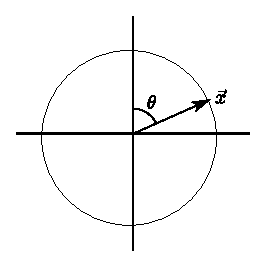
\includegraphics{figures/05clockwise-circle-problem.pdf}
  \end{center}
  \bigskip

\item[{\bf(V16.1g)}]

  Circle with radius 1 and center $(1,1)$ (it touches the $x$ and $y$ axes).
  Traversed infinitely often in counterclockwise fashion.
  \begin{center}
    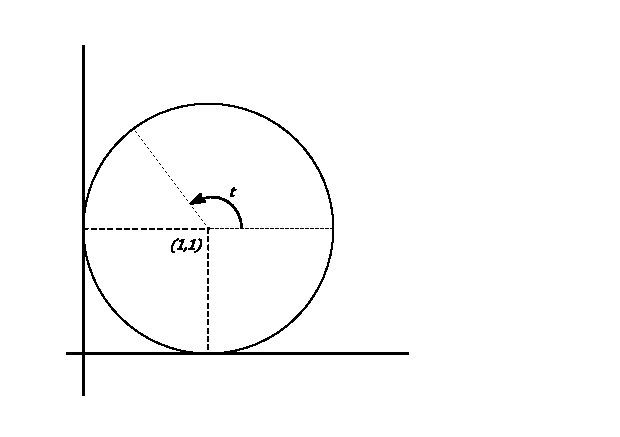
\includegraphics{figures/05circle-at-1-1-problem.pdf}
  \end{center}
  \bigskip

\item[{\bf(V16.1h)}]

  Without the $2$ this would be the standard unit circle (dashed curve below).
  Multiplying the $x$ component by $2$ stretches this circle to an ellipse.  So
  $(x(t), y(t))$ traces out an ellipse, infinitely often, counterclockwise.

  \begin{center}
    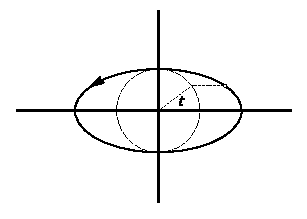
\includegraphics{figures/05ellipse-problem.pdf}
  \end{center}

  \bigskip

\item[{\bf(V16.1i)}]

  For each $y=t^3$ there is exactly one $t$, namely, $t=y^{1/3}$.  So the curve is
  a graph (with $x$ as a function of $y$ instead of the other way around).  It
  is the graph of $x=y^{2/3} = \sqrt[3]{y^2}$.
  \begin{center}
    \input figures/05neils-problem.tex
  \end{center}
  The curve is called \emph{Neil's parabola}.
  \bigskip

\item[{\bf(V16.6)}] Since $\sin^2t + \cos^2 t =1$ we have $y(t) = 1-x(t)$ on this curve.  The curve
  is a straight line and therefore its curvature is zero.
  \bigskip

\end{trivlist}
\noproblemfont
%\newpage
%%%%%%%%%%%%  GNU FDL  %%%%%%%%%%%%%%%
%%\input ../gfdl
\end{document}
